\title{\vspace{160px} \textbf{\huge{Telecommunication Theory}} \\\vspace{17.5px} \LARGE{Lab report 2}  \vspace{10px}}
\author{Alessandro Trigolo}
\date{October 2, 2023}

\begin{document}
\maketitle \newpage



\section*{Objective}
The goal of the lab work is to learn and try some more advanced modulation and detection techniques in order to make the transmitted signal more immune to the \textit{Gaussian White Noise} (\textbf{GWN}). Particularly, in the first task, the detection algorithm will be based on the average of the samples associated with a single symbol. This will make the transmission more reliable even with low values of the \textit{Signal to Noise Ratio} (\textbf{SNR}). 

In the second part of the lab work, the modulation technique will change to the \textbf{BASK} modulation (\textit{Binary Amplitude Shift Keying}). This modulation technique will focus on the frequency of the signal rather than its amplitude. Clearly, with this change, the detection algorithm has to be updated, otherwise it will lead to several detection errors. The new detection algorithm will rely on the signal's energy which is calculated as the integral of the square of the signal: this, in fact, represents the area between the time-axis and the signal itself.


% 
% 
\section*{Source code and plots}
The MATLAB source code produced in order to accomplish the laboratory goal is presented in the following section. Alongside the lines of code, there will be some explanatory comments for the purpose of making the source code more readable.
\lstset{style = MatLab}

\subsection*{Tasks 1 and 2}
Task 1 and task 2 asked to reorder the code of the first lab work to generate only one window which contains three specific plots:

\vspace{-5px}
\begin{enumerate}
\setlength{\itemsep}{-2px}
    \item The transmitted signal, is calculated with a simulation of the DAC, the \textit{Kroner} multiplication;
    \item The disturbed signal, is computed by adding the GWN to the original signal;
    \item The detected signal, is generated by comparing the disturbed signal with a threshold.
\end{enumerate}\vspace{-5px}
In order to place the three plots inside the same window it has been used the \texttt{subplot} function, as suggested in the lab guidelines.

\begin{lstlisting}
%% tasks 1 & 2
clc, clearvars, clear

SYMBOLS = 10; % number of symbols
s = randi(2, 1, SYMBOLS) - 1; % random sequence of 1 and 0


% --- Transmitted signal
SAMPLES_PER_SYMBOL = 100; % number of samples utilized per each symbol
s0 = ones(1, SAMPLES_PER_SYMBOL); 
sTx = kron(s, s0); % kroner multiplication simulating DAC

subplot(3, 1, 1), plot(sTx, 'b', 'Linewidth', 1), grid on; % draws the first plot
xlabel('Time, units'), ylabel('Signal'), title('Transmitted signal'), ylim([-.5, 1.5]); % adds labels and title


% --- Signal with GWN
SNR = 10; % dB

sRx = awgn(sTx, SNR); % adds noise to the transmitted signal
threshold = ( max(sTx) + min(sTx) ) / 2; % calculates the threshold 

subplot(3, 1, 2), plot(sRx, 'b'), grid on; % draws the second plot
xlabel('Time, units'), ylabel('Signal'), title('Disturbed signal'), ylim([min(sRx), max(sRx)]); % adds labels and title
hold on, plot([0, length(sTx)], [threshold, threshold], 'r', 'Linewidth', 1), hold off; % adds threshold red line


% --- Detected signal
sD = sRx > threshold; % regenerate the signal

subplot(3, 1, 3), plot(sD, 'b', 'Linewidth', 1); grid on; % draws the third plot
xlabel('Time, units'), ylabel('Signal'), title('Detected signal'); ylim([-.5, 1.5]); % adds labels and title
\end{lstlisting}

\begin{figure}[h!]
    \centering
    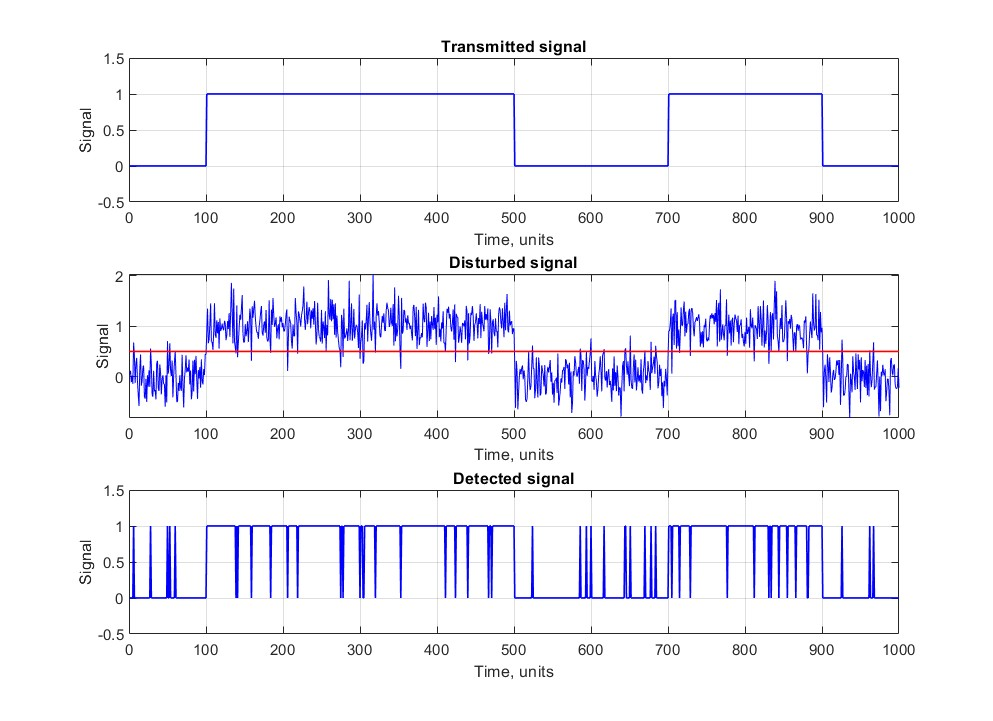
\includegraphics[width = \textwidth]{lab-2/imgs/task1&2.jpg}
\end{figure}

% 
\subsection*{Task 3}
In the third task, it was asked to modify the detection algorithm in order to reduce the error rate. Precisely, the disturbed signal has been split into 10 parts, one for every symbol, through the \texttt{reshape} function. Then, the detection algorithm was modified in such a way that, instead of comparing every sample with the threshold, the average value of 100 samples was compared to the threshold. This provides significant help with the noise-immunity of the signal because to have an error, the mean of the 100 samples has to be lower (or greater) than the threshold and this is highly improbable due to the fact that one of the properties of the GWN is that the average value $\mu \to 0$ as the number of samples increases to infinity.

The code for the first two plots is the same written for tasks 1 and 2 and consequently, in order to avoid unnecessary redundance, the following source code contains the changes done to draw the third plot excluding d the first two.

\begin{lstlisting}
%% Task 3

%      [ Same code of tasks 1 & 2 ]

% --- Detected signal
sRx = reshape(sRx, SAMPLES_PER_SYMBOL, SYMBOLS); % slice received signal into segments 
sD = mean(sRx) > threshold; % compare the mean of each column with the threshold  
sDvec = kron(sD,ones(1,SAMPLES_PER_SYMBOL)); 

subplot(3, 1, 3), stairs(sDvec, 'b', 'Linewidth', 1); grid on; % draws the third plot
xlabel('Time, units'), ylabel('Signal'), title('Detected signal'); ylim([-.5, 1.5]); % adds labels and title
\end{lstlisting}

% 
\subsection*{Task 4}
The fourth task required creating three graphs of the signals (the transmitted, disturbed, and detected signal) while varying the SNR at the following four values: 20, 10, 5, and -5. Precisely because each time the initial signal is generated randomly, every presented plot will have a different transmitted signal from the others.

In the first case, the signal is 100 times stronger than the GWN: the signal is so powerful that also by not changing the detection algorithm there are no problems regenerating the signal (as we saw in the previous lab work).

\begin{figure}[h!]
    \centering
    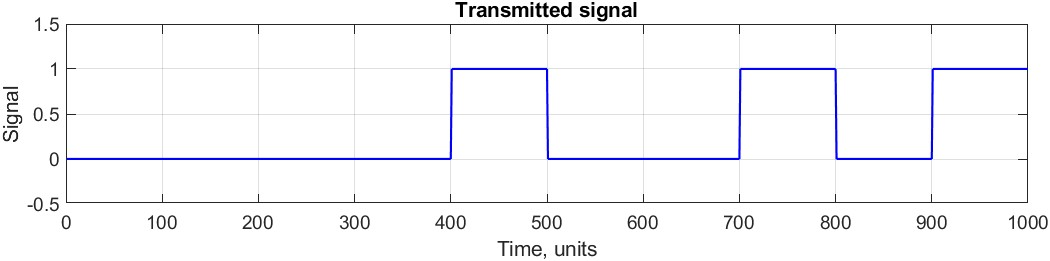
\includegraphics[width = .85\textwidth]{lab-2/imgs/task4.1_Transmitted.jpg}
\end{figure}
\vspace{-15px}
\begin{figure}[h!]
    \centering
    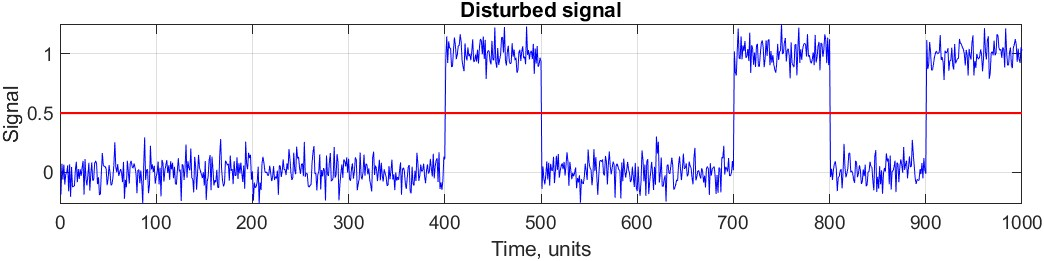
\includegraphics[width = .85\textwidth]{lab-2/imgs/task4.1_Noise.jpg}
\end{figure}
\vspace{-15px}
\begin{figure}[h!]
    \centering
    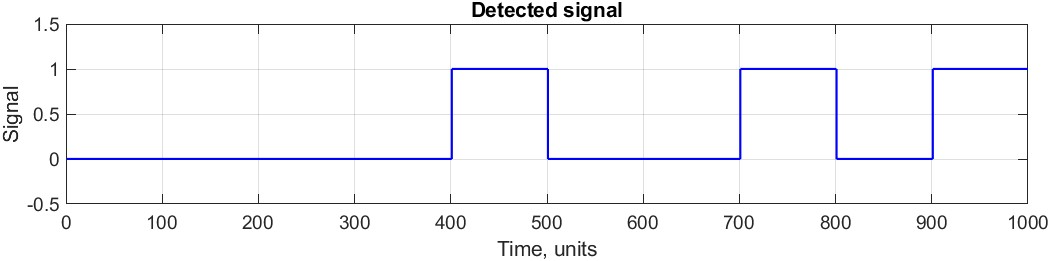
\includegraphics[width = .85\textwidth]{lab-2/imgs/task4.1_Detected.jpg}
\end{figure}

\FloatBarrier\noindent By setting the SNR value at 10dB the signal is 10 times stronger than the white noise. This could already provide several problems when no detection algorithm is applied to the receiver, as shown in the plot displayed in tasks 1 and 2. But this algorithm has no problems detecting the disturbed signal, as we can see in the following plots.

\begin{figure}[h!]
    \centering
    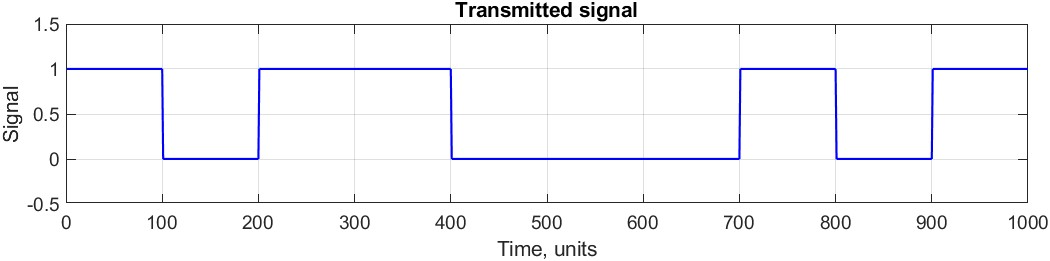
\includegraphics[width = .85\textwidth]{lab-2/imgs/task4.2_Transmitted.jpg}
\end{figure}
\vspace{-15px}
\begin{figure}[h!]
    \centering
    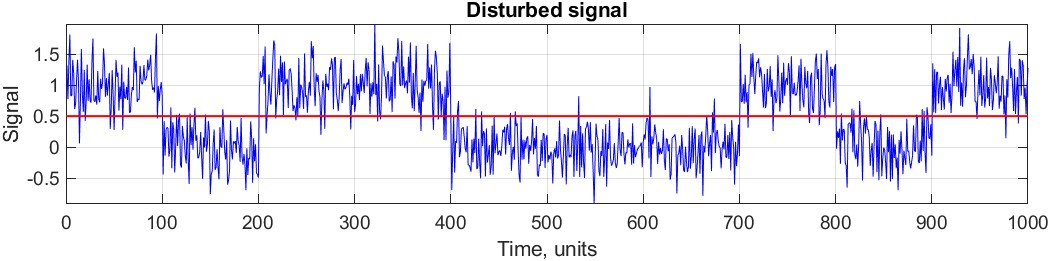
\includegraphics[width = .85\textwidth]{lab-2/imgs/task4.2_Noise.jpg}
\end{figure}
\vspace{-15px}
\begin{figure}[h!]
    \centering
    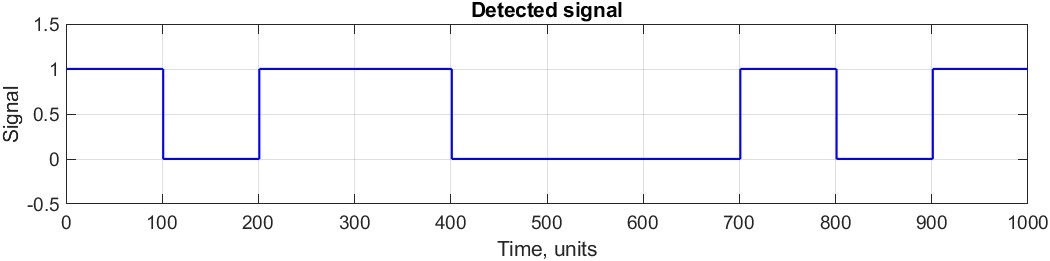
\includegraphics[width = .85\textwidth]{lab-2/imgs/task4.2_Detected.jpg}
\end{figure}

\FloatBarrier\noindent Setting the SNR to 5 means that the signal is a little more than 3 times stronger than the noise. By looking at the following figure, it is getting harder to understand what was the original signal by only observing the second plot; nevertheless, the detection algorithm is capable of regenerating the signal.

\begin{figure}[h!]
    \centering
    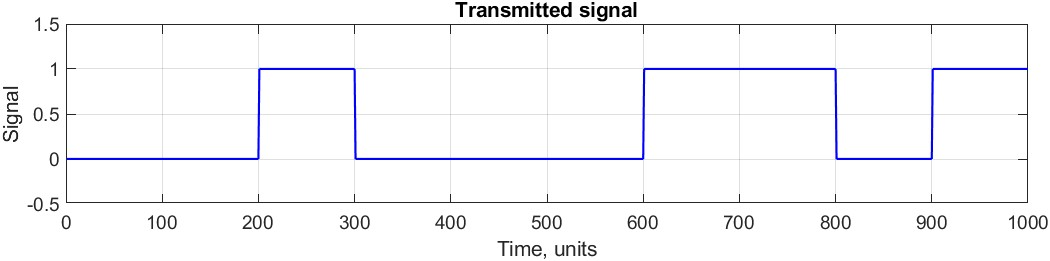
\includegraphics[width = .85\textwidth]{lab-2/imgs/task4.3_Transmitted.jpg}
\end{figure}
\vspace{-15px}
\begin{figure}[h!]
    \centering
    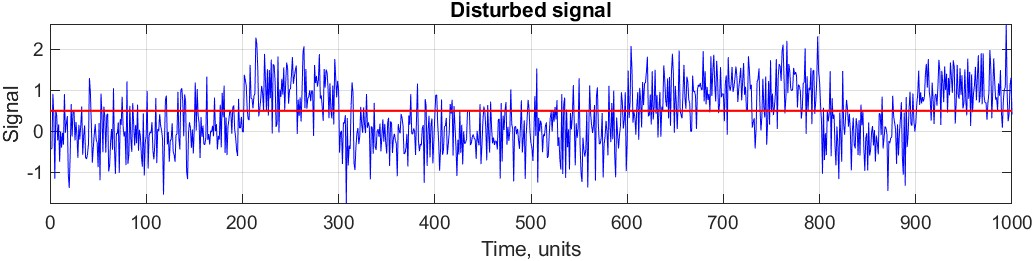
\includegraphics[width = .85\textwidth]{lab-2/imgs/task4.3_Noise.jpg}
\end{figure}
\vspace{-15px}
\begin{figure}[h!]
    \centering
    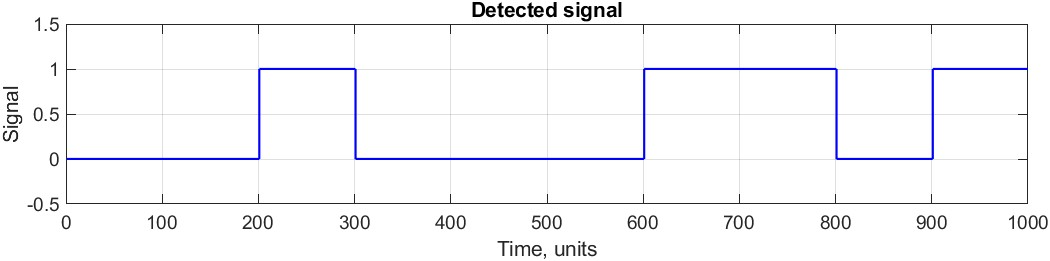
\includegraphics[width = .85\textwidth]{lab-2/imgs/task4.3_Detected.jpg}
\end{figure}

\FloatBarrier\noindent When the SNR reaches the value -5dB it means that the noise is more than 3 times stronger than the transmitted signal. Observing the plots underneath, it is almost impossible to detect the original signal by the human eye but with the detection algorithm, the signal is correctly regenerated. 

\begin{figure}[h!]
    \centering
    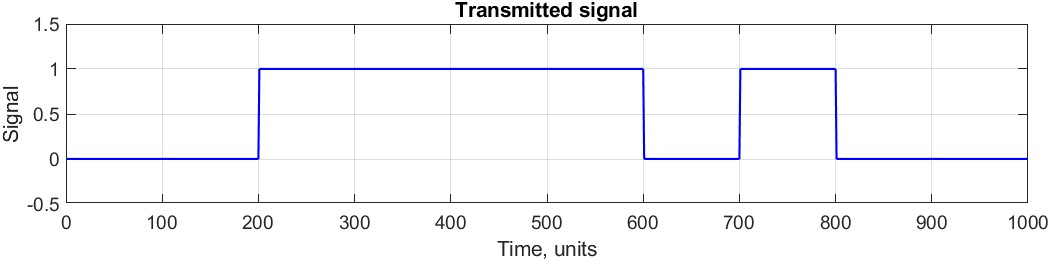
\includegraphics[width = .85\textwidth]{lab-2/imgs/task4.4_Transmitted.jpg}
\end{figure}
\vspace{-15px}
\begin{figure}[h!]
    \centering
    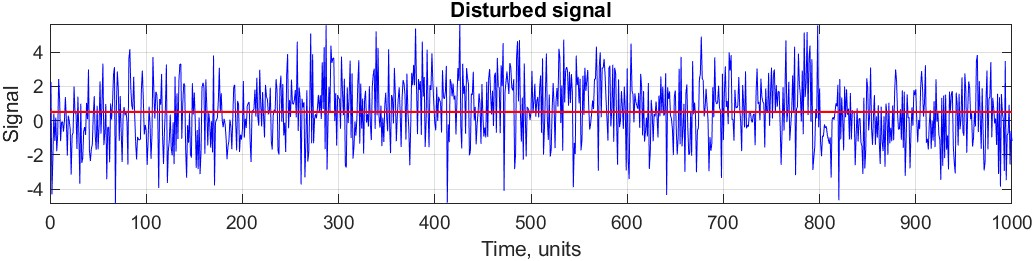
\includegraphics[width = .85\textwidth]{lab-2/imgs/task4.4_Noise.jpg}
\end{figure}
\vspace{-15px}
\begin{figure}[h!]
    \centering
    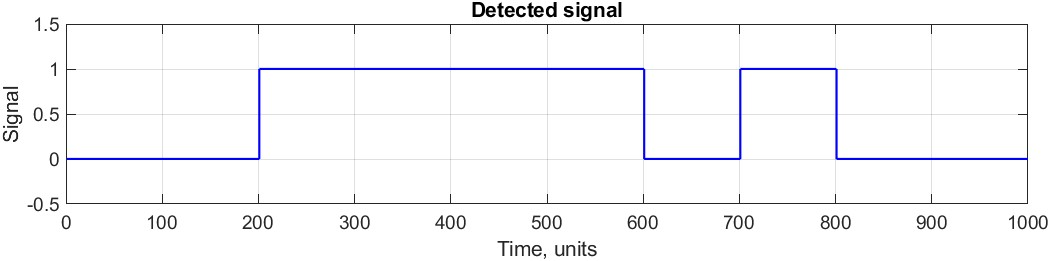
\includegraphics[width = .85\textwidth]{lab-2/imgs/task4.4_Detected.jpg}
\end{figure}

\FloatBarrier\noindent Nevertheless, by running the code shown in task 3 several times, there could be times when an error might occur. This is because the noise has a Gaussian distribution and, if we are unfortunate enough, it is possible to come upon some errors. In the following figure, the last \texttt{"1"} of the sequence is counted as a \texttt{"0"}.

\begin{figure}[h!]
    \centering
    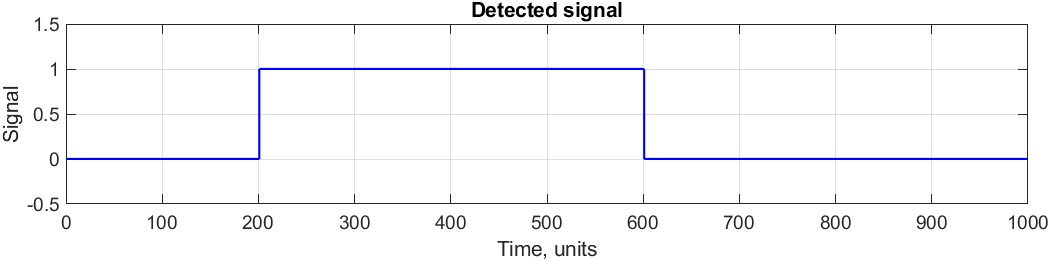
\includegraphics[width = .85\textwidth]{lab-2/imgs/task4.4_Detected_Error.jpg}
\end{figure}

% 
\subsection*{Task 5}
In task number five it was asked to increase the number of transmitted symbols from 10 to 10 thousand and then update the script with the purpose of counting the errors that occurred during the transmission. The following code only contains the script used to count the errors. The changes made to the source code and not displayed are the following:
\vspace{-5px}
\begin{enumerate}
\setlength{\itemsep}{-2px}
    \item The variable \texttt{SYMBOLS} has been set to \texttt{10000}.
    \item The \texttt{SNR} variable is set to \texttt{-5} in order to make some errors occur;
    \item In order to display only the first 25 symbols inside the \texttt{plot} function it has been inserted the limitation \texttt{sTx(1:25*SAMPLES\_PER\_SYMBOL)} instead of just the signal \texttt{sTx}. This update has been made in every plot: \texttt{sTx}, \texttt{sRx} and also \texttt{sDvec}.
    \item The first argument of the \texttt{plot} for the \texttt{threshold} was updated as follow: \texttt{[0, 25*SAMPLES\_PER\_SYMBOL]}.
\end{enumerate}
\vspace{-5px}

\begin{lstlisting}
%% Task 5

%      [ Same code of task 3 with little changes previously mentioned ] 

% Error calculation
errVec = (sD ~= s); % creates a vector containing the different bits between sD and s
errors = sum(errVec); % number of total errors
disp('Total errors: ' + errors); % displays the number of errors
\end{lstlisting}


\vspace{10px}\noindent As we can see from the following figure, the noise makes the signal impossible to detect by the human eye but, as already mentioned in task 4, the detection algorithm is able to regenerate the signal without errors.

\begin{figure}[h!]
    \centering
    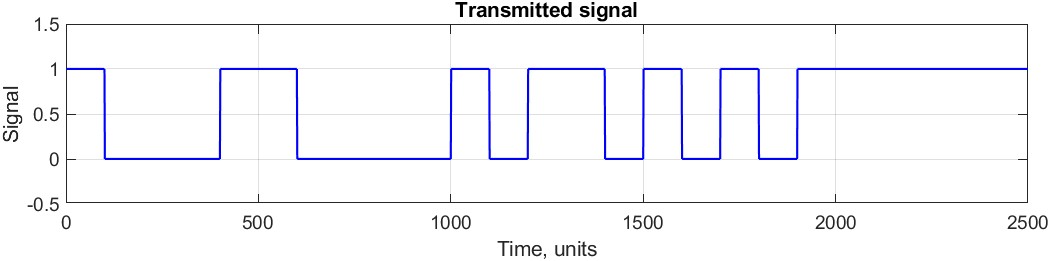
\includegraphics[width = \textwidth]{lab-2/imgs/task5_Transmitted.jpg}
\end{figure}
\vspace{-15px}
\begin{figure}[h!]
    \centering
    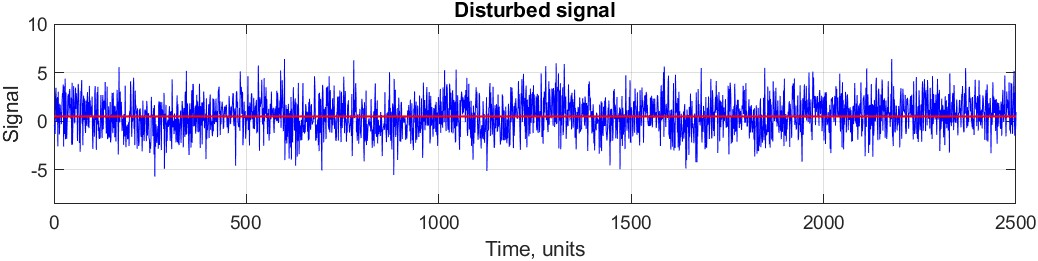
\includegraphics[width = \textwidth]{lab-2/imgs/task5_Noise.jpg}
\end{figure}
\vspace{-15px}
\begin{figure}[h!]
    \centering
    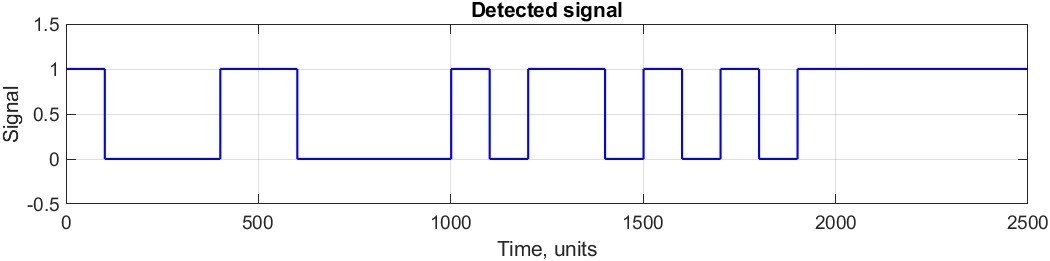
\includegraphics[width = \textwidth]{lab-2/imgs/task5_Detected.jpg}
\end{figure}

\FloatBarrier\noindent After running the code, on the command window, it is possible to notice that the overall number of errors that occurred during the transmission has been displayed:
\begin{verbatim}
                            Total errors: 26
                            >> 
\end{verbatim}
In this case, with a significantly weak signal (3 times weaker than the GWN) in 10 thousand symbols, only 26 have been received wrong, which means that 99.974\% of the symbols have been detected correctly. This is a remarkable result, considering that the noise was three times stronger than the original signal.


% 
\subsection*{Task 6}
The sixth task asked to change the carrier type, from unipolar to BASK: this means that now when a \texttt{"1"} occurs, instead of increasing the signal amplitude from 0 Volts to 1 Volt, a sine wave is transmitted. In order to accomplish this new modulation, it was necessary to change the first part of the code previously utilized as follows:

\begin{lstlisting}
%% Task 5
clc, clearvars, clear

SYMBOLS = 10000;
s = randi(2, 1, SYMBOLS) - 1; % random sequence of 1 and 0

SAMPLES_PER_SYMBOL = 100;


% --- Transmitted signal
SAMPLES_PER_PERIOD = 20; % number of samples per period
PERIODS = (0 : SAMPLES_PER_SYMBOL - 1 )/SAMPLES_PER_PERIOD; % calculates the number of periods for each symbol

s0 = sin(2 * pi * PERIODS); % BASK modulation: carrier is a sine wave
sTx = kron(s, s0); % kroner multiplication simulating DAC

subplot(3, 1, 1), plot( sTx(1:25*SAMPLES_PER_SYMBOL) , 'b', 'Linewidth', 1), grid on; % draws the first plot
xlabel('Time, units'), ylabel('Signal'), title('Transmitted signal'), ylim([-1.5, 1.5]); % adds labels and title

% [ Same code of task 5 ]
\end{lstlisting}

\noindent As we can see from the following figure, by running the code, the detected signal presents lots of errors if compared with the transmitted signal, even if the GWN is significantly weaker. 

\begin{figure}[h!]
    \centering
    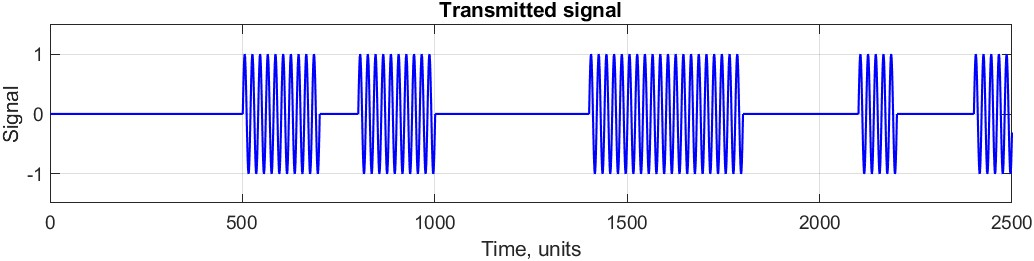
\includegraphics[width = \textwidth]{lab-2/imgs/task6_Transmitted.jpg}
\end{figure}
\vspace{-15px}
\begin{figure}[h!]
    \centering
    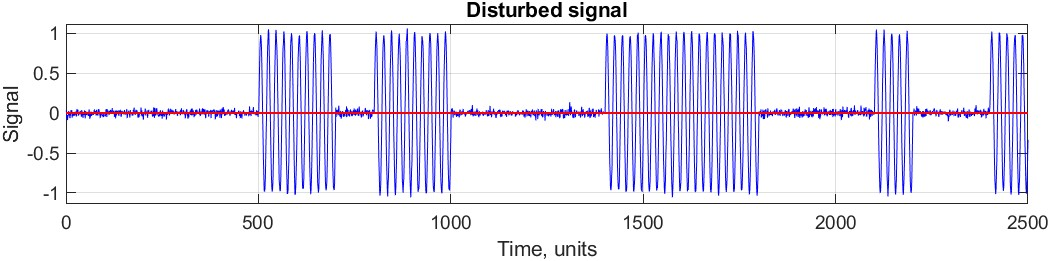
\includegraphics[width = \textwidth]{lab-2/imgs/task6_Noise.jpg}
\end{figure}
\vspace{-15px}
\begin{figure}[h!]
    \centering
    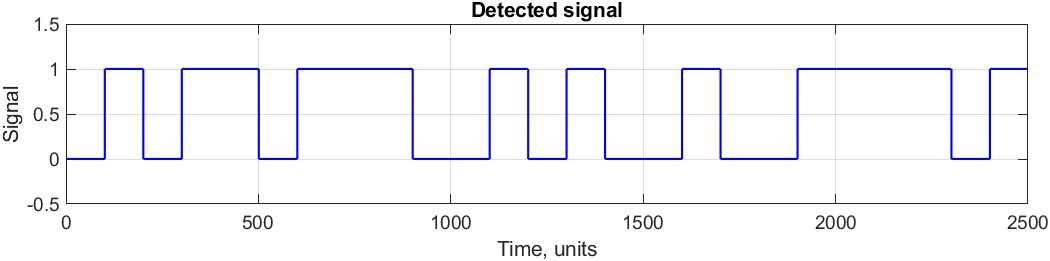
\includegraphics[width = \textwidth]{lab-2/imgs/task6_Detected.jpg}
\end{figure}

\FloatBarrier\noindent Sure enough, upon checking the number of errors that occurred during the transmission, out of 10 thousand symbols transmitted, almost half of them were wrongly detected:

\begin{verbatim}
                            Total errors: 4984
                            >> 
\end{verbatim}
This is due to the fact that, while the carrier signal has been changed, the detection algorithm hasn't. This has led to several errors during the regeneration of the signal because the average value of the period of a sine wave is 0.

% 
\subsection*{Task 7}
Task number 7 requested to modify the detection algorithm in order to regenerate the disturbed signal correctly. In this case, instead of calculating the average value of the samples it has been used the energy of the signal. Precisely the threshold in this case would be half of the energy of the carrier which is calculated through the scalar product between the carrier and itself with the \texttt{dot} function. In such a way the sum of every squared discrete carrier component has been calculated. The threshold is half of this sum. After calculating the threshold, the detecting algorithm compares the \textbf{correlation receiver} with the threshold.

Underneath the complete code produced for task number 7 is presented. It is noticeable that in this case the threshold red line has been removed because the energy, as the integral of the signal, cannot be represented as a line.

\begin{lstlisting}
%% Task 7

clc, clearvars, clear

SYMBOLS = 10000;
s = randi(2, 1, SYMBOLS) - 1; % random sequence of 1 and 0

SAMPLES_PER_SYMBOL = 100;


% --- Transmitted signal
SAMPLES_PER_PERIOD = 20; % number of samples per period
PERIODS = (0 : SAMPLES_PER_SYMBOL - 1 )/SAMPLES_PER_PERIOD; % calculates the number of periods for each symbol

s0 = sin(2 * pi * PERIODS); % carrier is a sine wave
sTx = kron(s, s0); % kroner multiplication simulating DAC

subplot(3, 1, 1), plot( sTx(1:25*SAMPLES_PER_SYMBOL) , 'b', 'Linewidth', 1), grid on; % draws the first plot
xlabel('Time, units'), ylabel('Signal'), title('Transmitted signal'), ylim([-1.5, 1.5]); % adds labels and title


% --- Signal with GWN
SNR = 5; % dB
sRx = awgn(sTx, SNR); % adds noise to the transmitted signal

subplot(3, 1, 2), plot(sRx(1:25*SAMPLES_PER_SYMBOL), 'b'), grid on; % draws the second plot
xlabel('Time, units'), ylabel('Signal'), title('Disturbed signal'), ylim([min(sRx), max(sRx)]); % adds labels and title


% --- Detected signal
threshold =  dot( s0, s0 ) / 2; % half of the carrier's energy

sRx = reshape(sRx, SAMPLES_PER_SYMBOL, SYMBOLS); % slice received signal into segments 

sD = (s0 * sRx) > threshold; % compares the with the threshold  

sDvec = kron(sD,ones(1,SAMPLES_PER_SYMBOL));

subplot(3, 1, 3), stairs(sDvec(1:25*SAMPLES_PER_SYMBOL), 'b', 'Linewidth', 1); grid on; % draws the third plot
xlabel('Time, units'), ylabel('Signal'), title('Detected signal'); ylim([-.5, 1.5]); % adds labels and title

% Error calculation
errVec = (sD ~= s); % creates a vector containing the different bits between sD and s
errors = sum(errVec); % number of total errors
disp("Total errors: " + errors); % displays the number of errors
\end{lstlisting}

% 
\subsection*{Task 8}
In this final task, it was asked to run the code produced in Task 7 and compare the results obtained by changing the SNR value, checking the errors and summarizing the results in a table. 

By setting SNR to 20, no errors occur during the telecommunication, as expected. Symbols can indeed be distinguished by examining only the second plot in the following figure. 

\begin{figure}[h!]
    \centering
    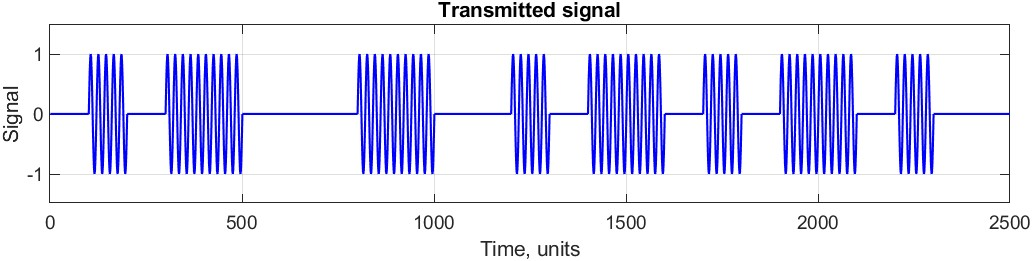
\includegraphics[width = .85\textwidth]{lab-2/imgs/task8.1_Transmitted.jpg}
\end{figure}
\vspace{-15px}
\begin{figure}[h!]
    \centering
    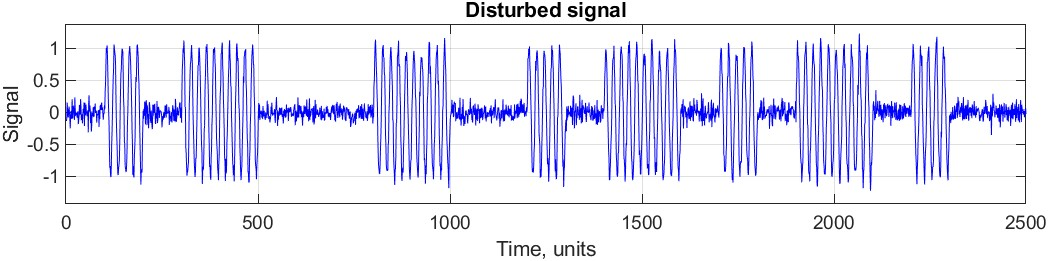
\includegraphics[width = .85\textwidth]{lab-2/imgs/task8.1_Noise.jpg}
\end{figure}
\vspace{-15px}
\begin{figure}[h!]
    \centering
    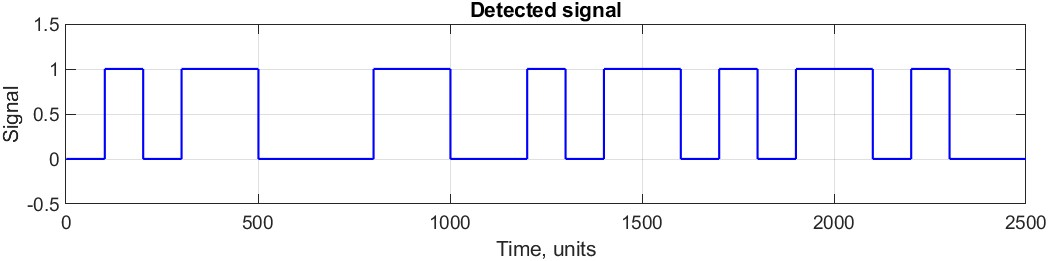
\includegraphics[width = .85\textwidth]{lab-2/imgs/task8.1_Detected.jpg}
\end{figure}

\FloatBarrier\noindent The same result has been reached also by setting the SNR to 10, meaning that the signal is now 10 times weaker than the previous transmission. Still, it is possible to detect, also by the human eye, the original signal in the second plot.

\begin{figure}[h!]
    \centering
    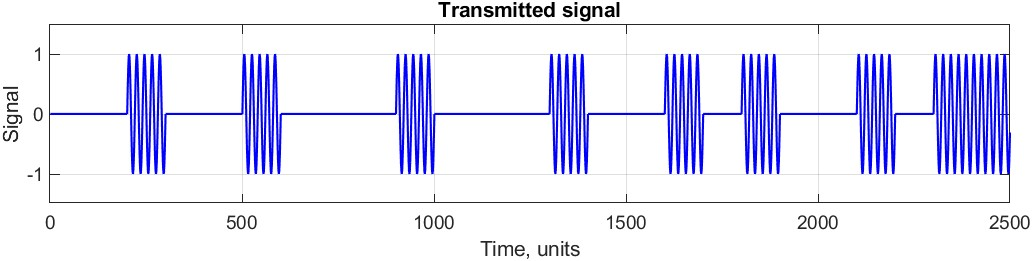
\includegraphics[width = .85\textwidth]{lab-2/imgs/task8.2_Transmitted.jpg}
\end{figure}
\vspace{-15px}
\begin{figure}[h!]
    \centering
    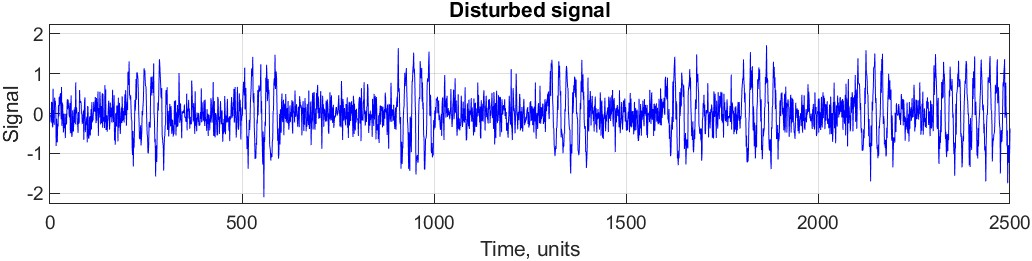
\includegraphics[width = .85\textwidth]{lab-2/imgs/task8.2_Noise.jpg}
\end{figure}
\vspace{-15px}
\begin{figure}[h!]
    \centering
    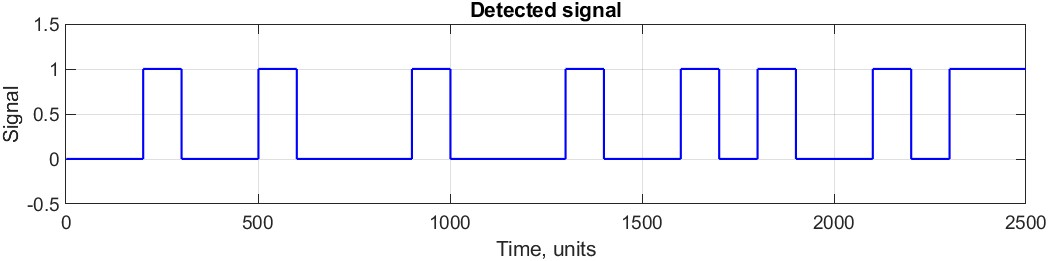
\includegraphics[width = .85\textwidth]{lab-2/imgs/task8.2_Detected.jpg}
\end{figure}

\FloatBarrier\noindent By halving the SNR to 5 the transmission didn't come upon any errors even though now the signal is not much stronger than the noise.

\begin{figure}[h!]
    \centering
    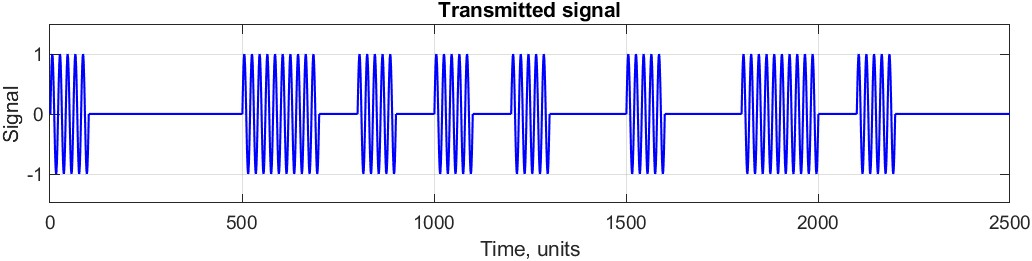
\includegraphics[width = .85\textwidth]{lab-2/imgs/task8.3_Transmitted.jpg}
\end{figure}
\vspace{-15px}
\begin{figure}[h!]
    \centering
    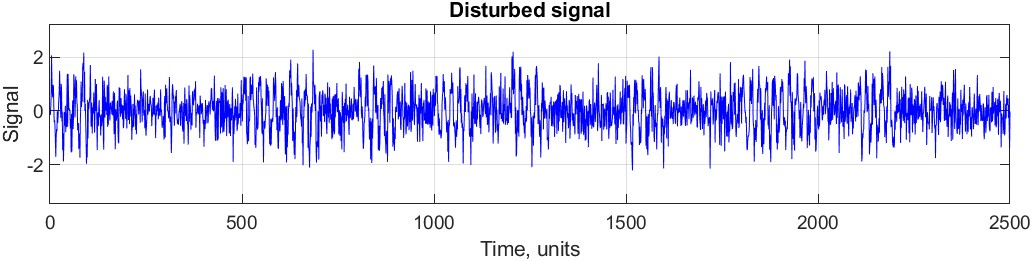
\includegraphics[width = .85\textwidth]{lab-2/imgs/task8.3_Noise.jpg}
\end{figure}
\vspace{-15px}
\begin{figure}[h!]
    \centering
    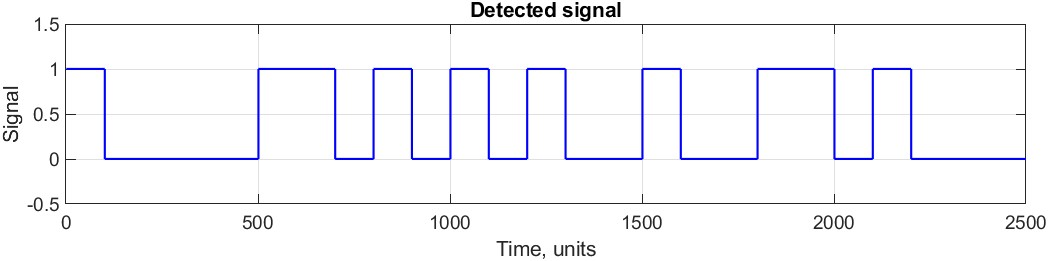
\includegraphics[width = .85\textwidth]{lab-2/imgs/task8.3_Detected.jpg}
\end{figure}

\FloatBarrier\noindent Some errors started to occur when the SNR was reduced to -5 meaning that the noise is more than 3 times stronger than the transmitted signal. Observing the following figure, the third and the fifth symbols are in fact different from the original signal.

\begin{figure}[h!]
    \centering
    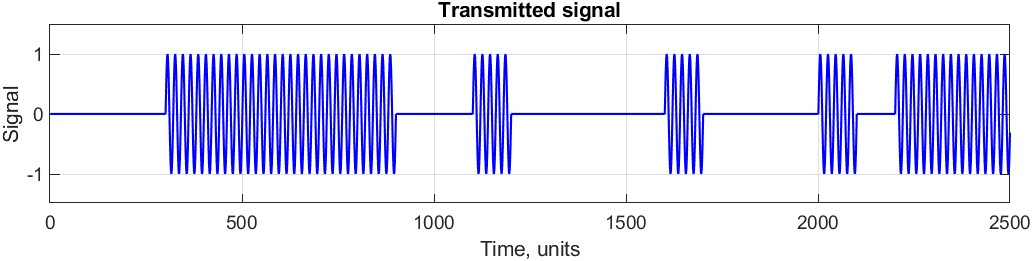
\includegraphics[width = .85\textwidth]{lab-2/imgs/task8.4_Transmitted.jpg}
\end{figure}
\vspace{-15px}
\begin{figure}[h!]
    \centering
    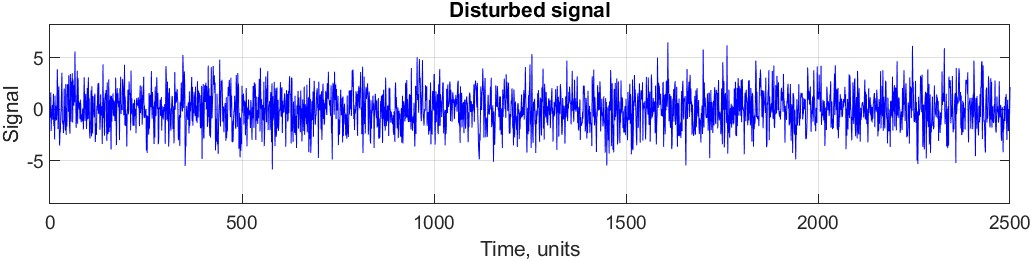
\includegraphics[width = .85\textwidth]{lab-2/imgs/task8.4_Noise.jpg}
\end{figure}
\vspace{-15px}
\begin{figure}[h!]
    \centering
    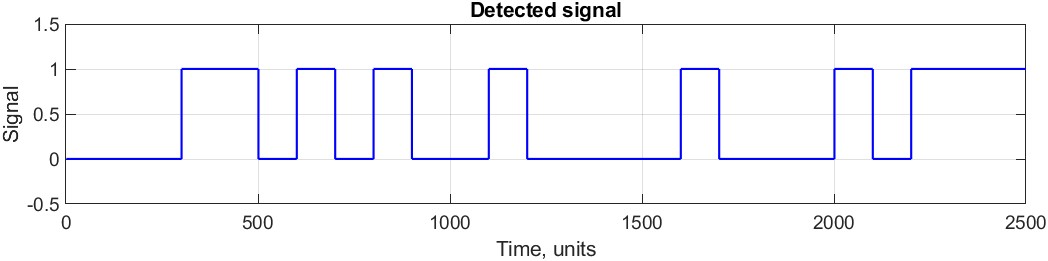
\includegraphics[width = .85\textwidth]{lab-2/imgs/task8.4_Detected_Error.jpg}
\end{figure}

\FloatBarrier\noindent When the SNR decreases to -10, meaning that the GWN is 10 times stronger than the signal, the errors start to become more frequent, as shown in the following plot.

\begin{figure}[h!]
    \centering
    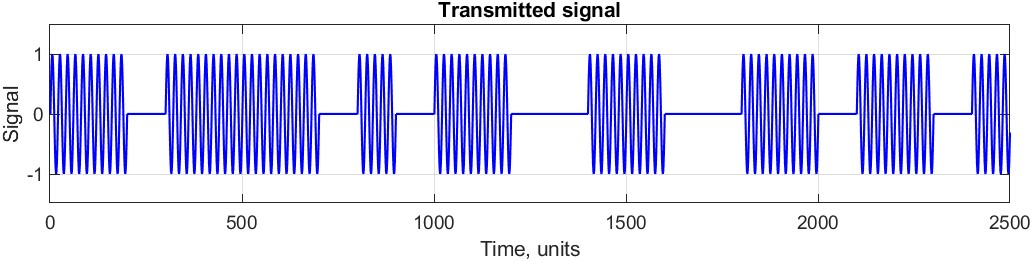
\includegraphics[width = .85\textwidth]{lab-2/imgs/task8.5_Transmitted.jpg}
\end{figure}
\vspace{-15px}
\begin{figure}[h!]
    \centering
    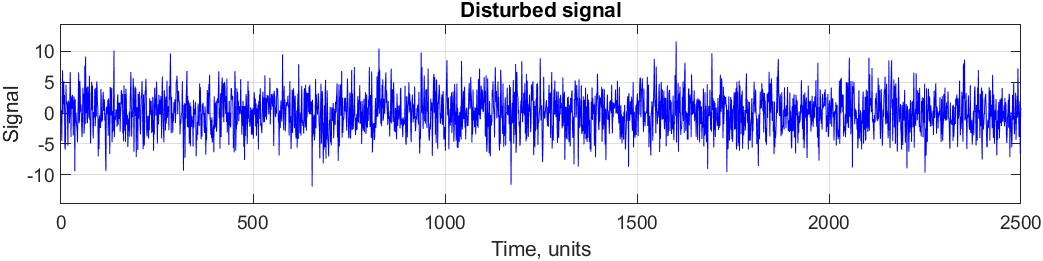
\includegraphics[width = .85\textwidth]{lab-2/imgs/task8.5_Noise.jpg}
\end{figure}
\vspace{-15px}
\begin{figure}[h!]
    \centering
    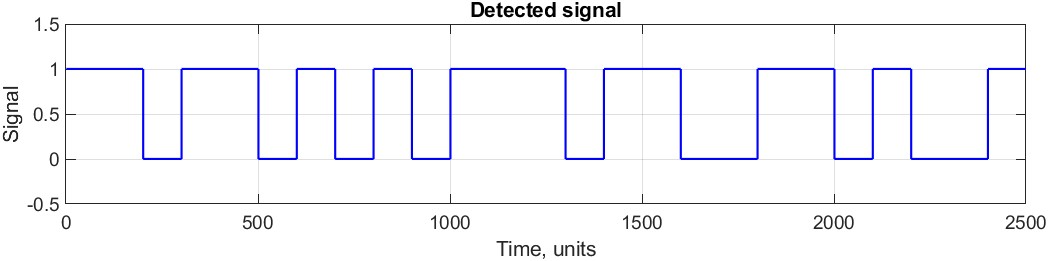
\includegraphics[width = .85\textwidth]{lab-2/imgs/task8.5_Detected_Error.jpg}
\end{figure}

\FloatBarrier\noindent Finally, when the signal becomes 100 times weaker than the white noise, meaning that the SNR reaches the value of -20, the errors are even more frequent. In fact, in the following figure, it is possible to notice that one of every three symbols is wrongly detected.

\begin{figure}[h!]
    \centering
    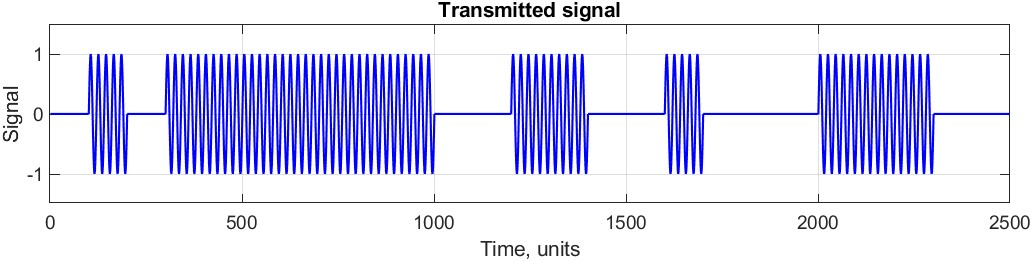
\includegraphics[width = .85\textwidth]{lab-2/imgs/task8.6_Transmitted.jpg}
\end{figure}
\vspace{-15px}
\begin{figure}[h!]
    \centering
    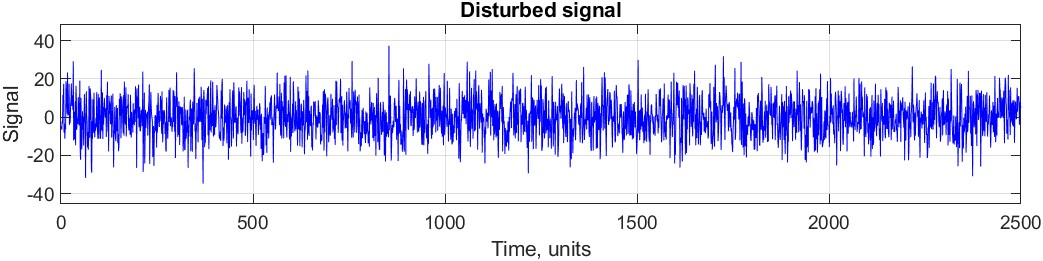
\includegraphics[width = .85\textwidth]{lab-2/imgs/task8.6_Noise.jpg}
\end{figure}
\vspace{-15px}
\begin{figure}[h!]
    \centering
    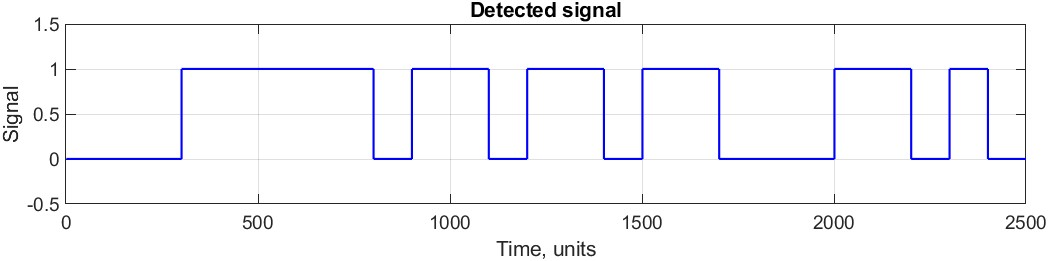
\includegraphics[width = .85\textwidth]{lab-2/imgs/task8.6_Detected_Error.jpg}
\end{figure}

\FloatBarrier\noindent The table below displays the number of errors that occurred as the SNR was varied during the transmission. Of course, when the noise starts to be stronger than the signal the errors begin to increase. When the SNR decreases to -20 the transmission becomes so disturbed that more than a third of the transmitted symbols are wrongly detected making the transmission unreliable. 

\begin{table}[h!]
    \centering
    \begin{tabular}{|c|c|} 
        \hline \textbf{SNR value} & \textbf{Number of errors}  \\\hline\hline
        
         20 & 0 \\
         10 & 0 \\
         5 & 0 \\
         -5 & 204 \\
         -10 & 1316 \\
         -20 & 3624 \\\hline
    \end{tabular}
\end{table}

% 
% 
\section*{Conclusions}
Through these simulations, we can conclude that both of the techniques make the transmission highly reliable and noise-immune. Specifically, by modifying the detection algorithm to average the samples of the symbol, it's evident that even with the SNR reduced to -5, only 26 symbols out of 10 thousand were wrongly detected, making the transmission nearly flawless despite the GWN being three times stronger than the signal.

In the second part of the lab work, when changing the modulation technique to BASK and subsequently updating the detection algorithm, the results obtained were essentially the same: the transmission is indeed flawless for SNR values greater than 5. However, as the noise begins to overpower the signal, errors start to increase, reaching 3600 out of 10 thousand errors during the transmission.

In conclusion, it is important to note that when the SNR is greater than zero, both the modulation techniques and algorithms utilized in the lab work led to optimal data transmission, resulting in zero errors out of 10 thousand transmitted symbols.





\end{document}